\section{Графический калькулятор}
\label{sec:a_graphical_calculator}

Вернёмся к нашему примеру с калькулятором, описанным в предыдущей главе о 
императивном программировании (\ref{sec:calculator_with_memory}). Создадим для 
него графический интерфейс, облегчающий использование.

Интерфейс реализует кнопки (цифры и функции) и экран для просмотра результата. 
Кнопка может быть нажата либо с использованием мыши, либо с клавиатуры. На 
рисунке \ref{fig:graphical_calculator} изображён будущий интерфейс.

\begin{figure}[h]
	\center{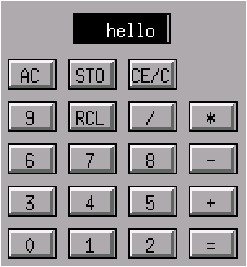
\includegraphics[scale=0.7]{drafts/book-ora018}}
	\caption{\label{fig:graphical_calculator}Графический калькулятор}
\end{figure}

Здесь мы вновь воспользуемся функцией рисования блоков, описанной на странице 
\ref{subsec:example_drawing_of_boxes_with_relief_patterns}. Определим следующий 
тип:

\begin{lstlisting}[language=OCaml]
# type etat_calc = 
  { e : etat; t : (box_config * touche * string ) list; v : box_config } ;;
\end{lstlisting}

В нем хранится состояние калькулятора, список блоков для каждой кнопки и блок 
для вывода результата. Так как мы хотим построить легко изменяемый калькулятор, 
поэтому создание интерфейса параметризовано списком из ассоциаций:

\begin{lstlisting}[language=OCaml]
# let descr_calc = 
  [  (Chiffre 0,"0");  (Chiffre 1,"1");    (Chiffre 2,"2");  (Egal, "=");
     (Chiffre 3,"3");  (Chiffre 4,"4");    (Chiffre 5,"5");  (Plus, "+"); 
     (Chiffre 6,"6");  (Chiffre 7,"7");    (Chiffre 8,"8");  (Moins, "-");
     (Chiffre 9,"9");  (MemoireOut,"RCL"); (Par, "/");       (Fois,  "*"); 
     (Off,"AC");       (MemoireIn, "STO"); (Clear,"CE/C") 
  ] ;;
\end{lstlisting}

\subsubsection{Создание блоков кнопок}

С помощью этого описания мы создаём список блоков. У функции \code{gen\_boxes} 
5 параметров: описание (\code{descr}), число колонок (\code{n}), расстояние 
между кнопками (\code{wsep}), расстояние между текстом и границами блока 
(\code{wsepint}), размер окантовки (\code{wbord}). Она возвращает список блоков 
кнопок и блок для вывода результата. Для вычисления расположения элементов, 
воспользуемся функцией \code{max\_xy} вычисляющей максимальные размеры списка 
пар целых чисел, а также функцию \code{max\_lbox} вычисляющую максимальное 
положение списка блоков.

\begin{lstlisting}[language=OCaml]
# let gen_xy vals comp o  = 
   List.fold_left (fun  a (x,y) -> comp (fst a) x,comp (snd a) y) o vals ;;
val gen_xy : ('a * 'a) list -> ('b -> 'a -> 'b) -> 'b * 'b -> 'b * 'b = <fun>
# let max_xy vals = gen_xy vals max (min_int,min_int);;
val max_xy : (int * int) list -> int * int = <fun>
# let max_boxl l = 
   let bmax (mx,my) b = max mx b.x, max my b.y
   in List.fold_left bmax  (min_int,min_int) l ;;
val max_boxl : box_config list -> int * int = <fun>
\end{lstlisting}

Ниже представлена главная функция \code{gen\_boxes}, создающая интерфейс.

\begin{lstlisting}[language=OCaml]
# let gen_boxes  descr n wsep wsepint wbord   = 
   let l_l = List.length descr in 
   let nb_lig = if l_l mod n = 0 then l_l / n else l_l / n + 1 in 
   let ls = List.map (fun (x,y) -> Graphics.text_size y) descr in
   let sx,sy = max_xy  ls in
   let sx,sy= sx+wsepint ,sy+wsepint  in 
     let r = ref [] in 
       for i=0 to l_l-1 do
         let px = i mod n and py = i / n in 
           let b = { x = wsep * (px+1) + (sx+2*wbord) * px  ; 
                     y = wsep * (py+1) + (sy+2*wbord) * py ;
                     w = sx; h = sy ; bw = wbord;
                     r=Top;
                     b1_col = grey1;  b2_col = grey3; b_col =grey2} 
           in r:= b::!r
       done;
       let mpx,mpy = max_boxl !r in 
       let upx,upy = mpx+sx+wbord+wsep,mpy+sy+wbord+wsep in
       let (wa,ha) = Graphics.text_size "        0" in 
         let v = { x=(upx-(wa+wsepint +wbord))/2 ; y= upy+ wsep;
                   w=wa+wsepint; h = ha +wsepint; bw = wbord *2; r=Flat ;
                   b1_col = grey1;  b2_col = grey3; b_col =Graphics.black} 
         in 
           upx,(upy+wsep+ha+wsepint+wsep+2*wbord),v,
           List.map2 (fun b (x,y) -> b,x,y ) (List.rev !r) descr;;
val gen_boxes :
  ('a * string) list ->
  int ->
  int ->
  int -> int -> int * int * box_config * (box_config * 'a * string) list =
  <fun>
\end{lstlisting}

\subsubsection{Взаимодействие}

Мы хотим воспользоваться скелетом определённым на странице 
\ref{subsec:program_skeleton}, для этого определим функции обработки клавиатуры 
и мыши. Функция обработки нажатий на клавиши клавиатуры очень проста; она 
передаёт символ, переведённый в тип \type{key}, функции калькулятора 
\code{transition}, затем выводит текст о состоянии калькулятора.

\begin{lstlisting}[language=OCaml]
# let f_clavier ec c = 
   transition ec.e (traduction c);
   draw_string_in_box Right (string_of_int ec.e.vaf) ec.v Graphics.white ;;
val f_clavier : etat_calc -> char -> unit = <fun>
\end{lstlisting}

Обработка мышиных событий немного сложней. Необходимо удостоверится, что нажатие 
было произведено на одну из кнопок калькулятора. Для этого, определим функцию, 
которая проверяющую положение на принадлежность блоку.

\begin{lstlisting}[language=OCaml]
# let mem (x,y) (x0,y0,w,h) = 
     (x >= x0) && (x< x0+w) && (y>=y0) && ( y<y0+h);;
val mem : int * int -> int * int * int * int -> bool = <fun>
# let f_souris ec x y = 
   try 
     let b,t,s = 
       List.find (fun (b,_,_) -> 
                    mem (x,y) (b.x+b.bw,b.y+b.bw,b.w,b.h)) ec.t
     in 
       transition ec.e t;
       draw_string_in_box Right (string_of_int ec.e.vaf ) ec.v Graphics.white
   with Not_found -> ();;
val f_souris : etat_calc -> int -> int -> unit = <fun>
\end{lstlisting}

Если функция \code{f\_mouse} нашла блок, которому соответствуют координаты 
нажатия, она передаёт соответствующую кнопку функции перехода, затем выводит 
результат. В противном случае эта функция ничего не делает.

Функция \code{f\_exc} обрабатывает исключения которые могут возникнуть во время 
выполнения программы.

\begin{lstlisting}[language=OCaml]
# let f_exc cs ex = 
  match ex with 
   Division_by_zero -> 
     transition cs.s Clear;
     erase_box cs.v;
     draw_string_in_box Right "Div 0" cs.v (Graphics.red)
 | Invalid_key -> ()
 | Key_off -> raise End
 | _  -> raise ex;;
val f_exc : calc_state -> exn -> unit = <fun>
\end{lstlisting}

В случае деления на ноль, эта функция обнулеят состояние калькулятора и выводит 
сообщение об ошибке. Неправильная клавиша просто--напросто игнорируется. И 
наконец, исключение \code{Key\_off} возбуждает исключение \code{End} выхода из 
цикла скелета программы.

\subsubsection{Инициализация и выход}

При инициализации калькулятора необходимо вычислить размер окна. Следующая 
функция генерирует нужную графическую информацию, для этого она использует 
список кнопка-текст и возвращает размер главного окна.

\begin{lstlisting}[language=OCaml]
# let create_e t = 
     Graphics.close_graph ();
     Graphics.open_graph " 10x10";
     let mx,my,v,lb = gen_boxes t 4 4 5 2 in 
     let s = {dce=0; dta = false; doa = Egal; vaf = 0; mem = 0}   in 
       mx,my,{e=s; t=lb;v=v};;
val create_e : (touche * string) list -> int * int * etat_calc = <fun>
\end{lstlisting}

Функция инициализации использует результат предыдущей функцию. 

\begin{lstlisting}[language=OCaml]
# let f_init mx my ec () = 
       Graphics.close_graph();
       Graphics.open_graph (":0 "^(string_of_int mx)^"x"^(string_of_int my));
       Graphics.set_color grey2;
       Graphics.fill_rect 0 0 (mx+1) (my+1);
       List.iter (fun (b,_,_) -> draw_box b) ec.t;
       List.iter 
         (fun (b,_,s) -> draw_string_in_box Center s b Graphics.black) ec.t ;
       draw_box ec.v;
       draw_string_in_box Right "hello" ec.v (Graphics.white);;
val f_init : int -> int -> etat_calc -> unit -> unit = <fun>
\end{lstlisting}

Функция выхода закрывает окно.

\begin{lstlisting}[language=OCaml]
# let f_fin e () = Graphics.close_graph();;
val f_fin : 'a -> unit -> unit = <fun>
\end{lstlisting}

Функция \code{go}, параметризованная описанием, запускает цикл ожидания событий.

\begin{lstlisting}[language=OCaml]
# let go descr = 
   let mx,my,e = create_e descr in
     squel (f_init mx my e) (f_fin e) (f_clavier e) (f_souris e) (f_exc e);;
val go : (touche * string) list -> unit = <fun>
\end{lstlisting}

Вызов \code{go descr\_calc} соответствует изображению 
\ref{fig:graphical_calculator}.
